% !TeX spellcheck = en_US
\documentclass[12pt]{article}
\usepackage[T1]{fontenc}
\usepackage[utf8]{inputenc}
\usepackage{amsmath,amsthm,amsfonts,amssymb,amscd}
\usepackage[lining,semibold,scaled=1.05]{ebgaramond}     
%\usepackage[cmintegrals,cmbraces]{newtxmath}
% Use FUCKING GARAMOND
\usepackage{hyperref}
\hypersetup{
	colorlinks,
	linkcolor={red!50!black},
	citecolor={blue!50!black},
	urlcolor={blue!80!black}
}
\urlstyle{same}
\usepackage[ebgaramond]{newtxmath}
\usepackage{xparse}
\usepackage{minted}
\usepackage{graphicx}                    
% Publication quality tables          
% Driver-independent color extensions
\usepackage[margin=1in]{geometry}           
% Customize document dimensions        
% all 4 margins to be either 1 inch or 1.5 cm
\usepackage{mathtools}           

% Creating circuits        
% Print exactly what you type in
\usepackage[us]{datetime} 
% Various time format
\usepackage{blindtext}
\usepackage{bbding}
\usepackage[scr=euler,cal=dutchcal,frak=euler,bb=dsfontserif,bbsymbols]{mathalfa}
\usepackage{bbm}
\usepackage{bm}
\usepackage{multirow}
\usepackage{multicol}
\usepackage[x11names,table]{xcolor}
\usepackage[shortlabels]{enumitem}   
\usepackage{standalone}
\usepackage{microtype}
\usepackage{censor}
\usepackage[backend=biber,style=alphabetic]{biblatex}
\usepackage{courier}
\usepackage{movement-arrows}
\usepackage{algorithm}
\usepackage{algpseudocode}
\usepackage[makeroom]{cancel}
\usepackage{tcolorbox}
\tcbuselibrary{skins,raster,theorems,listings,minted}
\usepackage{mathtools}
\usepackage{soul}
\usepackage{multicol}
\usepackage{caption}
\usepackage{wrapfig}
\usepackage{authblk}
\usepackage{float}
\usepackage{fontawesome5}
\usepackage{tikz}
\usetikzlibrary{positioning}
\usetikzlibrary{shapes.geometric,arrows,patterns,arrows.meta, bending,calc,matrix, shadings,intersections,shadows,decorations,fit,backgrounds,circuits.ee.IEC,shapes.callouts}
\newcounter{dummy}



\definecolor{dkgreen}{rgb}{0,0.6,0}
\definecolor{dred}{rgb}{0.545,0,0}
\definecolor{dblue}{rgb}{0,0,0.545}
\definecolor{lgrey}{rgb}{0.9,0.9,0.9}
\definecolor{gray}{rgb}{0.4,0.4,0.4}
\definecolor{darkblue}{rgb}{0.0,0.0,0.6}
\DeclareMathOperator*{\argmax}{arg\,max}
\DeclareMathOperator*{\argmin}{arg\,min}


\renewcommand{\labelitemi}{$\textcolor{SteelBlue4}{\bullet}$}
\renewcommand{\labelitemii}{$\textcolor{blue}{\cdot}$}
\renewcommand{\labelitemiii}{$\textcolor{SkyBlue4}{\diamond}$}
\renewcommand{\labelitemiv}{$\textcolor{SkyBlue4}{\ast}$}

\newcommand{\enf}[1]{\textcolor{DodgerBlue3}{\textbf{#1}}} %enf sta per enfasi
\let\emph\enf
\newcommand{\sott}[1]{\setulcolor{SkyBlue3}\ul{#1}}
\let\underline\sott

\newcommand{\prob}{\mathbb{P}}
\newcommand\independent{\protect\mathpalette{\protect\independenT}{\perp}}
\newcommand{\ev}{\mathbb{E}}
\def\independenT#1#2{\mathrel{\rlap{$#1#2$}\mkern2mu{#1#2}}}
\newcommand{\Z}{\mathbb{Z}}
\newcommand{\R}{\mathbb{R}}
\newcommand{\N}{\mathbb{N}}
\newcommand{\T}{\mathbb{T}}
\newcommand{\Tbar}{\overline{\T}}
\newcommand{\A}{\mathscr{A}}
\newcommand{\Nstar}{\N^{*}}
\newcommand{\Rext}{\overline{\R}}
\newcommand{\io}{\text{ i.o.}}
\newcommand{\normale}{\mathcal{N}}
\newcommand{\equalexpl}[1]{%
	\underset{\substack{\uparrow\\\mathrlap{\text{\vspace{-3cm}\hspace{-1em}#1}}}}{=}}
\newcommand{\dif}{\mathop{}\!\mathrm{d}}
\newcommand{\convas}{\xrightarrow[]{\text{a.s.}}}
\newcommand{\convpr}{\xrightarrow[]{\pr}}
\newcommand{\convd}{\xrightarrow[]{\text{d}}}
\newcommand{\convlp}{\xrightarrow[]{\lp}}
\newcommand{\lone}{L^{1}}
\newcommand{\convw}{\xrightarrow[]{\mathrm{weak}}}
\newcommand{\as}{\text{ a.s.}}
\newcommand{\asstnr}{\sim N(0,1)}
%\def\checkmark{\tikz\fill[scale=0.4](0,.35) -- (.25,0) -- (1,.7) -- (.25,.15) -- cycle;} 
\newcommand{\dx}{\dif x}
\newcommand{\dy}{\dif y}
\newcommand{\dt}{\dif t}
\newcommand{\du}{\dif u}
\newcommand{\ds}{\dif s}
\newcommand{\dw}{\dif\omega}
\newcommand{\dz}{\dif z}
\newcommand{\dmu}{\dif\mu}
\newcommand{\dpr}{\dif\pr}
\newcommand{\E}{\mathscr{E}}
\newcommand{\B}{\mathscr{B}}
\newcommand{\F}{\mathscr{F}}
\newcommand{\G}{\mathscr{G}}
\newcommand{\HS}{\mathscr{H}}
\newcommand{\Zn}{\mathscr{Z}}
\newcommand{\D}{\mathscr{D}}
\newcommand{\xbar}{\overline{X}}
\newcommand{\rbar}{\overline{\R}}
\newcommand{\ybar}{\overline{Y}}
\newcommand{\xxbar}{\overline{\xbar}}
\newcommand{\xtilde}{\widetilde{X}}
\newcommand{\ifonly}{\underline{if and only if}}
\newcommand{\ang}[1]{\langle#1\rangle}

\newcommand{\ubracketthin}[1]{\underbracket[0.3pt]{#1}}

\newcommand*\circled[1]{\tikz[baseline=(char.base)]{
		\node[shape=circle,draw,
		shading=ball, ball color=SkyBlue1!70,
		,inner sep=1.5pt] (char) {\scriptsize\bfseries #1};}}
\newcommand{\circnum}{\protect\circled{\arabic*}}
\newcommand{\circlet}{\protect\circled{\alph*}}	
\newcommand{\bbg}[1]{%
	\ooalign{$#1$\cr\raisebox{-.2pt}{$#1$}\cr\raisebox{.2pt}{$#1$}\cr\textcolor{white}{$\mkern0.2mu#1$}}%
}
\newcommand{\leb}{\bbg{\lambda}}

%i comandi di MERDA di stefano
\newcommand{\ra}{\rightarrow}
\newcommand{\iy}{\infty}
\newcommand{\mE}{\mathbb{E}}
\newcommand{\mP}{\mathbb{P}}
\newcommand{\mB}{\mathcal{B}(\mathbb{R})}
\newcommand{\mL}{\mathbb{L}}
\newcommand{\ninfty}{n\to$\infty$}
\newcommand{\tinfty}{t\to$\infty$}
\newcommand{\xinfty}{x\to$\infty$}
\newcommand{\yinfty}{y\to$\infty$}
\newcommand{\mLL}{\mathbb{L}^2(0,T)}
\newcommand{\mR}{\mathbb{R}}
\newcommand{\mC}{\mathcal{C}}
\newcommand{\mRd}{\mathbb{R}^d}
\newcommand{\mN}{\mathbb{N}}
%\newcommand{\m1}{\mathbf{1}}
\newcommand{\mF}{\mathcal{F}}
\newcommand{\mM}{\mathcal{M}}
\newcommand{\mW}{\mathcal{W}}
\newcommand{\mV}{\mathcal{V}}
\newcommand{\mA}{\mathcal{A}}
\newcommand{\mez}{\frac{1}{2}}
\newcommand{\intT}{\int_{0}^{T}}
\newcommand{\nN}{n \in \mathbb{N}}
\newcommand{\mmN}{\mathcal{N}}
\newcommand{\BM}{(B_t)_{t\geq 0}}
\newcommand{\PX}{(X_t)_{t\geq 0}}
\newcommand{\var}{\mathbb{V}\!\mathrm{ar}\,}
\newcommand{\cov}{\mathbb{C}\mathrm{ov}\,}
\newcommand{\lp}{L^{p}}
\newcommand{\BMF}{\left((B_t)_{t\geq 0},\mathcal{F}_t \right)}
\newcommand{\mFt}{\mathcal{F}_t}
\newcommand{\every}{\forall\,}
\newcommand{\dyadic}{\mathcal{d}}
\newcommand{\norm}[1]{\left|\negthinspace\left|#1\right|\negthinspace\right|}
\newcommand{\pr}{\mathbb{P}}
\newcommand{\indi}{\mathbb{1}}
\newcommand{\trns}[1]{{#1}^{\scriptscriptstyle\mathsf{T}}}
\newcommand{\iid}{\stackrel{\mathrm{iid}}{\sim}}
\newcommand{\unmezz}{\frac{1}{2}}
\newcommand{\sa}{$\sigma$-algebra}	\newcommand{\rv}{random variable}
\newcommand{\prefacename}{Preface}
\newcommand{\cinlar}{Çinlar }
\newenvironment{preface}{
	\vspace*{\stretch{2}}
	{\noindent \bfseries \huge\color{SkyBlue4} \prefacename}
	\begin{center}
		% \phantomsection \addcontentsline{toc}{chapter}{\prefacename} % enable this if you want to put the preface in the table of contents
		\thispagestyle{plain}
	\end{center}%
}
{\vspace*{\stretch{5}}}


\newenvironment{closethedeal}{
	\vspace*{\stretch{2}}
	{\noindent \bfseries \huge\color{SkyBlue4} That's all, folks}
	\begin{center}
		% \phantomsection \addcontentsline{toc}{chapter}{\prefacename} % enable this if you want to put the preface in the table of contents
		\thispagestyle{plain}
	\end{center}%
}
{\vspace*{\stretch{5}}}
\pgfkeys{%
	/calloutquote/.cd,
	width/.code                   =  {\def\calloutquotewidth{#1}},
	position/.code                =  {\def\calloutquotepos{#1}}, 
	author/.code                  =  {\def\calloutquoteauthor{#1}},
	/calloutquote/.unknown/.code   =  {\let\searchname=\pgfkeyscurrentname
		\pgfkeysalso{\searchname/.try=#1,                                
			/tikz/\searchname/.retry=#1},\pgfkeysalso{\searchname/.try=#1,
			/pgf/\searchname/.retry=#1}}
}  


\newcommand\calloutquote[2][]{%
	\pgfkeys{/calloutquote/.cd,
		width               = 5cm,
		position            = {(0,-1)},
		author              = {}}
	\pgfqkeys{/calloutquote}{#1}                   
	\node [rectangle callout,draw,callout relative pointer={\calloutquotepos},text width=\calloutquotewidth,/calloutquote/.cd,
	#1] (tmpcall) at (0,0) {#2};
	\node at (tmpcall.pointer){\calloutquoteauthor};    
}  		


\newcommand\lemmethink[2][]{%
	\pgfkeys{/calloutquote/.cd,
		width               = 5cm,
		position            = {(0,-1)},
		author              = {}}
	\pgfqkeys{/calloutquote}{#1}                   
	\node [cloud callout,draw,callout relative pointer={\calloutquotepos},text width=\calloutquotewidth,/calloutquote/.cd,
	#1] (tmpcall) at (0,0) {#2};
	\node at (tmpcall.pointer){\calloutquoteauthor};    
}  											


\renewcommand\leq\leqslant
\renewcommand\geq\geqslant		
\setlength\parindent{0pt}

%%%%%%%%%%%%%%%%%%%%%%%%%%%%%%%%%%%%%%%%%%%%%%%%%%%%%%%%%%%%%%
%%%%%%%%%%%%%%%%%%%%%%%%%%%%%%%%%%%%%%%%%%%%%%%%%%%%%%%%%%%%%%
\usemintedstyle{monokai}
\definecolor{codeBg}{HTML}{282822}
\newenvironment{py}
{\VerbatimEnvironment
	\begin{minted}[
		bgcolor=codeBg,
		breaklines,
		fontsize=\footnotesize
		]
		{python}}
	{\end{minted}}

	%\newmintinline[bluecode]{c++}{\color{codeblue}}
	
\newcommand{\pyinl}[1]{\mintinline[bgcolor=black!40]{python}{#1}}
%%%%%%%%%%%%%%%%%%%%%%%%%%%%%%%%%%%%%%%%%%%%%%%%%%%%%%%%%%%%%%

%%%%%%%%%%%%%%%%%%%%%%%%%%%%%%%%%%%%%%%%%%%%%%%%%%%%%%%%%%%%%%%
\definecolor{UM_Brown}{HTML}{3D190D}
\definecolor{UM_DarkBlue}{HTML}{2264B0}
\definecolor{UM_LightBlue}{HTML}{1CA9E1}
\definecolor{UM_Orange}{HTML}{fEB415}
\addbibresource{biblio.bib}




\tikzstyle{startstop} = [rectangle, rounded corners, minimum width=3cm, minimum height=1cm,text centered, draw=black, fill=red!30]
\tikzstyle{io} = [trapezium, trapezium left angle=70, trapezium right angle=110, minimum width=3cm, minimum height=1cm, text centered, draw=black, fill=blue!30]
\tikzstyle{process} = [rectangle, minimum width=3cm, minimum height=1cm, text centered, draw=black, fill=orange!30]
\tikzstyle{decision} = [diamond, minimum width=3cm, minimum height=1cm, text centered, draw=black, fill=green!30]
\tikzstyle{arrow} = [thick,->,>=stealth]

\begin{document}
	\textcolor{UM_Brown}{
		\begin{center}
			\textbf{\Large Stochastic Processes}\\
			\vspace{5pt}
			Homework 1 \\
			\vspace{5pt}
			\textbf{M.S. in Stochastics and Data Science}\\
			\vspace{20pt}
			\textit{Niccolò Disassonia} 863128 \\
			\textit{Varaga Haghoubians} 1088805\\
			\textit{Lorenzo Sala} 943481\\
			\vspace{5pt}
			\today
		\end{center}
		\vspace{10pt}
		\hrule
	}
	
	
	
	
	%%%%%%%%%%%%%%% NEW SECTION %%%%%%%%%%%%%%% 
	\section*{Exercise 1}
	Let ${\{X(s)\}}_{0\leq s\leq 1}$ be Brownian bridge in $[0,1]$ such that $X(0)=X(1)=0$ and let 
	\begin{equation*}
		f(x,s|y,\tau)=\frac{\partial}{\partial x}\pr(X(s)<x|X(\tau)=y)
	\end{equation*}
	be the transition probability density function of the Brownian motion associated to the Brownian Bridge.
	\begin{enumerate}
		\item Prove that the transition probability density function $\varphi(x,t|y,\tau)$ of the Brownian bridge is given by 
		\begin{equation*}
			\varphi(x,t|y,\tau)=\frac{f(x,t|y,\tau)f(0,1|x,t)}{f(0,1|y,\tau)}.
		\end{equation*}
		\item Let $T_a$ be the first passage time of the brownian brdige through the boundary $s>0$. Determine the first passage time probability density function of the considered brownian bridge.
		\item How does the result change when the boundary is time dependent ($a(t)>0$)?
	\end{enumerate}
	\subsection*{Solution}
	\begin{enumerate}
		\item According to the given definition, we should say that
		\begin{equation*}
			\varphi(x,t|y,\tau)=\frac{\partial}{\partial x}\pr(X(t)<x|X(\tau)=y,X(1)=0).
		\end{equation*}
		This is the probability density function of reaching level $x$ at time $t$ knowing that at time $\tau$ we reached $y$ \textit{and} at time 1 we must be in 0.
		
		By the definition of conditional probability we know that 
		\begin{equation*}
			\pr(A|B,C)=\frac{\pr(A,B|C)}{\pr(B|C)}
		\end{equation*}
		So by setting
		\begin{equation*}
			\begin{array}{c}
				A=\{X(t)<x\}\\
				B=\{X(1)=0\}\\
				C=\{X(\tau)=y\}
			\end{array}
		\end{equation*}
		we get
		\begin{equation*}
			\pr(X(t)<x|X(\tau)=y,X(1)=0)=\frac{\pr(X(t)<x,X(1)=0|X(\tau)=y)}{\pr(X(1)=0|X(\tau)=y)}.
		\end{equation*}
		Differentiating with respect to $x$ we obtain
		\begin{equation*}
			\varphi(x,t|y,\tau)=\frac{\frac{\partial}{\partial x}\pr(X(t)<x,X(1)=0|X(\tau)=y)}{\pr(X(1)=0|X(\tau)=y)}.
		\end{equation*}
		\begin{comment}	
			At the same time we know that 
			\begin{equation*}
				\pr(A,B|C)=\pr(A|B,C)\pr(B|C)
			\end{equation*}
			so, using the events we defined earlier, we can rewrite the numerator of the right hand side of the above equation as
			\begin{equation*}
				\pr(X(t)<x,X(1)=0|X(\tau)=y)=\pr(X(t)<x|X(1)=0,X(\tau)=y)\pr(X(1)=0|X(\tau)=y).
			\end{equation*}
			If we differentiate with respect to $x$ we get
			\begin{align*}
				\frac{\partial}{\partial x}\pr(X(t)<x,X(1)=0|X(\tau)=y)&=\pr(X(1)=0|X(\tau)=y)\frac{\partial}{\partial x}\pr(X(t)<x|X(1)=0,X(\tau)=y)
			\end{align*}
		\end{comment}
		Now, think about the fact that $X(t)$ is a Browmian Motion: we know that it has strong Markov property. Therefore we can ``split'' the process in two: instead of considering only one process reaching $x$ at time $t$ and $0$ at time $1$ starting from $y$ at time $\tau$, we consider one process reaching level $x$ at time $t$ starting from $y$ at time $\tau$ and another reaching 0 at time 1 starting from $x$ at time $t$. This makes sense because the probability of going from $(x,t)$ to $(1,0)$ is not dependent on the probability of being in $(y,\tau)$ because of the strong Markov property. Using, as well, independence between increments of Brownian motion, we get
		\begin{equation*}
			\pr(X(t)<x|X(\tau)=y,X(1)=0)=\frac{\pr(X(t)<x|X(\tau)=y)\pr(X(1)=0|X(t)=x)}{\pr(X(1)=0|X(\tau)=y)}
		\end{equation*}
		These are all cumulative density functions, but we want to apply this result to the continuous setting we are working in.
		\begin{equation*}
			\ubracketthin{\frac{\partial}{\partial x}\pr(X(t)<x|X(\tau)=y,X(1)=0)}_{\varphi(x,t|y,\tau)}=\frac{f(x,t|y,\tau)f(0,1|x,t)}{f(0,1|y,\tau)}.
		\end{equation*}
		\item
		Let $T_a = \inf\{ s>0 : X(s) = a\}$ be the {first passage time} at which the Brownian Bridge (started at 0 and conditioned to be at 0 again at time 1) first hits the level $a > 0$. We want to determine the probability density function of $T_a$ over the interval $0 < t < 1$.
		Recall that, for a {standard Brownian Motion} (without conditioning on the endpoint), the probability density of the first passage time to level $a>0$ is known to be
		\[
		g_{T_a}^{(BM)}(t)
		\;=\;
		\frac{a}{\sqrt{2\pi\,t^{3}}}
		\exp\Bigl\{-\tfrac{a^{2}}{2\,t}\Bigr\}.
		\]
		In our case, $X(t)$ is a Brownian Bridge, i.e.\ we are imposing the condition $X(1)=0$. Equivalently, we are looking for
		\[
		\pr\!\bigl(T_a < t \,\big|\; X(1)=0\bigr).
		\]
		By the strong Markov property, before hitting $a$, $X(t)$ behaves like an unconditioned Brownian Motion. However, to remain consistent with $X(1)=0$ \textit{after} hitting $a$, we account for the probability that, starting at $a$ at time $t$, the process transitions to $0$ at time $1$. 
		The transition density of a standard Brownian Motion with variance $\sigma^2=1$ and drift $\mu=0$ is given by
		\[
		f(x,t \,|\, x_0,t_0)
		\;=\;
		\frac{1}{\sqrt{2\pi\,(t-t_0)}} \;
		\exp\!\Bigl\{-\tfrac{(x - x_0)^{2}}{2\,(t-t_0)}\Bigr\}.
		\]
		In particular, for going from $a$ at time $t$ to $0$ at time $1$:
		\[
		f\bigl(0,1 \,\big|\; a,t\bigr)
		\;=\;
		\frac{1}{\sqrt{2\pi\,(1-t)}}\;
		\exp\Bigl\{-\tfrac{(0 - a)^2}{2\,(1-t)}\Bigr\}
		\;=\;
		\frac{1}{\sqrt{2\pi\,(1-t)}}\;
		\exp\!\Bigl\{-\tfrac{a^{2}}{2\,(1-t)}\Bigr\}.
		\]
		Meanwhile, the unconditional (for $X(1)$) density at time 1 (starting from 0 at time 0) is $f\bigl(0,1 \,\big|\; 0,0\bigr) = \tfrac{1}{\sqrt{2\pi}}$.
		By Fortet’s equation (or the standard conditional-density argument), we get
		\[
		\frac{\partial}{\partial t}\,\Pr\!\bigl(T_a < t \,\big|\; X(1)=0\bigr)
		\;=\;
		g_{T_a}^{(BM)}(t)
		\;\times\;
		\frac{f\bigl(0,1 \,\big|\; a,t\bigr)}{f\bigl(0,1 \,\big|\; 0,0\bigr)}.
		\]
		Substituting the expressions above yields
		\[
		\frac{\partial}{\partial t}\,\Pr\bigl(T_a < t \mid X(1)=0\bigr)
		= \frac{a}{\sqrt{2\pi\,t^{3}}}\,\exp\!\Bigl(-\tfrac{a^{2}}{2\,t}\Bigr)
		\times \frac{\tfrac{1}{\sqrt{2\pi\,(1-t)}}\,\exp\!\Bigl(-\tfrac{a^{2}}{2\,(1-t)}\Bigr)}
		{\tfrac{1}{\sqrt{2\pi}}}
		\]
		\[
		= \frac{a}{2\pi\,\sqrt{t^{3}\,(1-t)}}\;
		\exp\!\Bigl(-\tfrac{a^{2}}{2}\bigl(\tfrac{1}{t}+\tfrac{1}{1-t}\bigr)\Bigr).
		\]
		
		Hence, the probability \textit{density} function of $T_a$ under the Brownian Bridge condition is
		\[
		g_{T_a}(t)
		\;=\;
		\frac{a}{2\pi\,\sqrt{t^{3}\,(1-t)}}\;
		\exp\!\Bigl\{-\tfrac{a^{2}}{2}\,\tfrac{1}{t\,(1-t)}\Bigr\},
		\quad 0 < t < 1.
		\]
		
		\noindent
		This result confirms that one must account both for the first hitting time density of an unconditioned Brownian Motion and for the fact that the process, after hitting $a$, must still end up back at $0$ at time $1$.
		
		\item For time-dependent boundaries, we know that the Fortet equation is still valid:
		\begin{equation*}
			f(a(t),t|X(t_{0})=0)=\int_{0}^{t}\dif\tau g(a(\tau),\tau|x_{0})f(a(t),t|a(\tau),\tau)
		\end{equation*}
		Where $g_{T_{a(\tau)}}(\tau|0)$ is the First Passage Time density for reaching the boundary $a(\tau)$ at time $\tau$, starting from 0.
		
		For the Brownian Bridge with a time-dependent boundary, we need to modify our approach from part 2. The First Passage Time density becomes:
		\begin{equation*}
			\begin{aligned}
				g_{T_{a(t)}}(t) 
				&= \frac{a(t)}{2\pi\sqrt{t^3(1-t)}} 
				\exp\!\Bigl(-\tfrac{a(t)^2}{2}\,\tfrac{1}{t(1-t)}\Bigr) \\[6pt]
				&\quad + \frac{1}{2\pi\sqrt{t^3(1-t)}} 
				\exp\!\Bigl(-\tfrac{a(t)^2}{2}\,\tfrac{1}{t(1-t)}\Bigr)
				\;\cdot\; \frac{\partial a(t)}{\partial t} 
				\;\cdot\; \frac{a(t)}{t(1-t)}.
			\end{aligned}
		\end{equation*}
		
		
		The additional term accounts for the rate of change of the boundary. If $a(t)$ is increasing, the probability of hitting the boundary decreases, and if $a(t)$ is decreasing, the probability increases.
		
		In summary, the time-dependent boundary introduces an additional term in the First Passage Time density that depends on the rate of change of the boundary function $a(t)$.
		So the probability of $\tau$ is not affected.
	\end{enumerate} 
	\section*{Exercise 2}
	Consider a standard Brownian Motion.
	
	\begin{enumerate}
		\item For $0 < u < u+v < u+v+w$ with $u,v,w > 0$ evaluate
		\begin{equation*}
			\ev[B(u)B(u+v)B(u+v+w)].
		\end{equation*}
		
		\item For $0 < u < u+v < u+v+w$ with $u,v,w > 0$ evaluate
		\begin{equation*}
			\ev[B(u)B(u+v)|B(u+v+w)].
		\end{equation*}
		
		\item Evaluate the covariance of $U(t) = e^{-t}B(e^{2t})$ and of $V(t) = (1-t)B(\frac{t}{1-t})$.
	\end{enumerate}
	
	\subsection*{Solution}
	
	\begin{enumerate}
		\item We have to evaluate 
		\begin{equation*}
			\ev(B(u)B(u+v)B(u+v+w)).
		\end{equation*}
		We call:
		\begin{equation*}
			\begin{array}{l}
				B(u)=X\\
				B(u+v)-B(u)=Y\\
				B(u+v+w)-B(u+v)=Z.
			\end{array}
		\end{equation*}
		
		
		We will need this to express the various Brownian motions as increments of each other, so that we can use the independence property. If we write
		\begin{align*}
			B(u+v)&=\ubracketthin{B(u+v)-B(u)}_{Y}+\ubracketthin{B(u)}_{X}=Y+X\\
			B(u+v+w)&=\ubracketthin{B(u+v+w)-B(u+v)}_{Z}+\ubracketthin{B(u+v)-B(u)}_{Y}+\ubracketthin{B(u)}_{Z}=X+Y+Z
		\end{align*}
		then our problem becomes
		\begin{align*}
			\ev\left[X(X+Y)(X+Y+Z)\right]&=\ev\left[X^{3}+X^{2}Y+X^{2}Z+X^{2}Y+XY^{2}+XYZ\right]\\
			&=\ev\left[X^{3}+2X^{2}Y+X^{2}Z+XY^{2}+XYZ\right]\\
			&=\ubracketthin{\ev\left[X^{3}\right]}_{\scriptscriptstyle\mathclap{\text{$=0$ 3rd moment of a normal}}}+2\ubracketthin{\ev\left[X^{2}Y\right]}_{X\independent Y}+\ubracketthin{\ev\left[X^{2}Z\right]}_{X\independent Z}+\ubracketthin{\ev\left[XY^{2}\right]}_{X\independent Y}+\ubracketthin{\ev\left[XYZ\right]}_{X\independent Y\independent Z}\\
			&=0+2\ubracketthin{\ev\left[X^{2}\right]\ev\left[Y\right]}_{0}+\ubracketthin{\ev\left[X^{2}\right]\ev[Y]}_{0}+\ubracketthin{\ev\left[X\right]\ev\left[Y^{2}\right]}_{0}\\&+\ubracketthin{\ev[X]\ev[Y]\ev[Z]}_{0}\\
			&=0.
		\end{align*}
		\item For $0 < u < u+v < u+v+w$ with $u,v,w > 0$, we need to evaluate $\ev[B(u)B(u+v)|B(u+v+w)]$.
		
		To solve this problem, we need to use the properties of conditional expectation and the fact that Brownian Motion is a Gaussian process.
		
		For a Gaussian process, the conditional distribution of any subset of variables given another subset is also Gaussian. The conditional mean and covariance can be computed using the formulas for conditional multivariate normal distributions.
		Compute the covariance matrix for the three processes $B(u), B(u+v), B(u+v+w)$:
		
		\begin{equation*}
			\Sigma = \begin{bmatrix}
				\var(B(u)) & \cov(B(u), B(u+v)) & \cov(B(u), B(u+v+w)) \\
				\cov(B(u+v), B(u)) & \var(B(u+v)) & \cov(B(u+v), B(u+v+w)) \\
				\cov(B(u+v+w), B(u)) & \cov(B(u+v+w), B(u+v)) & \var(B(u+v+w))
			\end{bmatrix}
		\end{equation*}
		
		For Brownian Motion, we have:
		\begin{align*}
			\var(B(t)) &= t \\
			\cov(B(s), B(t)) &= \min(s, t) \text{ for } s, t \geq 0
		\end{align*}
		
		Therefore:
		\begin{equation*}
			\Sigma = \begin{bmatrix}
				u & u & u \\
				u & u+v & u+v \\
				u & u+v & u+v+w
			\end{bmatrix}
		\end{equation*}
		
		Let's denote $X = \begin{pmatrix}
			B(u)\\
			B(u+v)
		\end{pmatrix}$ and $Y = B(u+v+w)$. We know that $(X, Y)$ follows a multivariate normal distribution with mean vector $\mu = (0, 0)$.
		
		For a multivariate normal distribution, the conditional expectation is:
		\begin{equation*}
			\ev[X|Y] = \mu_X + \Sigma_{XY}\Sigma_{YY}^{-1}(Y - \mu_Y)
		\end{equation*}
		
		In our case we can obtain the needed quantities by subdividing the $\Sigma$ matrix:
		\begin{center}
			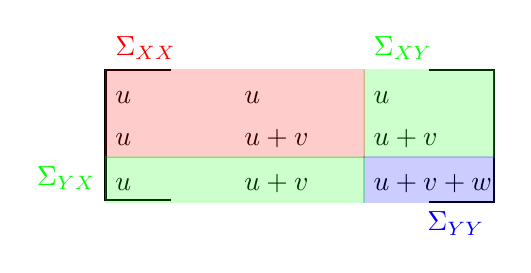
\begin{tikzpicture}[
				strip/.style = {
					draw=#1,%color
					line width=1em, opacity=0.2,
					line cap=round ,% only if you like them ...
				},
				]
				\matrix (mtrx)  [matrix of math nodes,
				column sep=0em,   
				nodes={text height=2ex,text width=4em}]
				{
					u & u & u \\
					u & u+v & u+v \\
					u & u+v & u+v+w \\
				};
				\draw[thick] (mtrx-1-1.north) -| (mtrx-3-1.south west) 
				-- (mtrx-3-1.south);
				\draw[thick] (mtrx-1-3.north) -| (mtrx-3-3.south east)
				-- (mtrx-3-3.south);
				\path[draw,fill,opacity=0.2,red]
				(mtrx-1-1.north west) rectangle (mtrx-2-2.south east) node[opacity=1,anchor=south west,pos=0]{$\Sigma_{XX}$};;
				\path[draw,shorten <=-1mm,fill,opacity=0.2,green]
				(mtrx-1-3.north west) rectangle (mtrx-2-3.south east) node[opacity=1,anchor=south west,pos=0]{$\Sigma_{XY}$};
				\path[draw,shorten <=-1mm,fill,opacity=0.2,green]
				(mtrx-3-1.north west) rectangle (mtrx-3-2.south east) node[opacity=1,anchor=north east,pos=0]{$\Sigma_{YX}$};
				\path[draw,shorten <=-1mm,fill,opacity=0.2,blue]
				(mtrx-3-3.north west) rectangle (mtrx-3-3.south east) node[opacity=1,anchor=north east,pos=1]{$\Sigma_{YY}$};
			\end{tikzpicture}
		\end{center}
		So the quantities we need are:
		\begin{align*}
			\mu_X &= (0, 0) \\
			\Sigma_{XY} &= \begin{pmatrix} u \\ u+v \end{pmatrix} \\
			\Sigma_{YY}^{-1} &= \frac{1}{u+v+w} \\
			\mu_Y &= 0
		\end{align*}
		
		Therefore:
		\begin{align*}
			\ev\left[\begin{pmatrix}
				B(u)\\ B(u+v)
			\end{pmatrix}\Big|B(u+v+w) = z\right] &= (0, 0) + \begin{pmatrix} u \\ u+v \end{pmatrix} \cdot \frac{1}{u+v+w} \cdot (z - 0) \\
			&= \begin{pmatrix} \frac{u}{u+v+w} \\ \frac{u+v}{u+v+w} \end{pmatrix} \cdot z
		\end{align*}
		
		This means:
		\begin{align*}
			\ev[B(u)|B(u+v+w) = z] &= \frac{u}{u+v+w} \cdot z \\
			\ev[B(u+v)|B(u+v+w) = z] &= \frac{u+v}{u+v+w} \cdot z
		\end{align*}
		
		Now, to find $\ev[B(u)B(u+v)|B(u+v+w)]$, we need to compute the conditional covariance as well:
		\begin{equation*}
			\cov(X|Y) = \Sigma_{XX} - \Sigma_{XY}\Sigma_{YY}^{-1}\Sigma_{YX}
		\end{equation*}
		
		In our case:
		\begin{align*}
			\Sigma_{XX} &= \begin{pmatrix} u & u \\ u & u+v \end{pmatrix} \\
			\Sigma_{XY}\Sigma_{YY}^{-1}\Sigma_{YX} &= \begin{pmatrix} u \\ u+v \end{pmatrix} \cdot \frac{1}{u+v+w} \cdot \begin{pmatrix} u & u+v \end{pmatrix} \\
			&= \frac{1}{u+v+w} \begin{pmatrix} u^2 & u(u+v) \\ (u+v)u & (u+v)^2 \end{pmatrix}
		\end{align*}
		
		Therefore:
		\begin{align*}
			\cov(X|Y) &= \begin{pmatrix} u & u \\ u & u+v \end{pmatrix} - \frac{1}{u+v+w} \begin{pmatrix} u^2 & u(u+v) \\ (u+v)u & (u+v)^2 \end{pmatrix} \\
			&= \begin{pmatrix} u - \frac{u^2}{u+v+w} & u - \frac{u(u+v)}{u+v+w} \\ u - \frac{(u+v)u}{u+v+w} & (u+v) - \frac{(u+v)^2}{u+v+w} \end{pmatrix}
		\end{align*}
		
		The conditional covariance between $B(u)$ and $B(u+v)$ given $B(u+v+w) = z$ is:
		\begin{align*}
			\cov(B(u), B(u+v)|B(u+v+w) = z) &= u - \frac{u(u+v)}{u+v+w} \\
			&= u\left(1 - \frac{u+v}{u+v+w}\right) \\
			&= u\left(\frac{u+v+w-(u+v)}{u+v+w}\right) \\
			&= u\left(\frac{w}{u+v+w}\right) \\
			&= \frac{uw}{u+v+w}
		\end{align*}
		
		Now, using the formula for the expectation of a product:
		\begin{align*}
			\ev[B(u)B(u+v)\mid B(u+v+w) = z]
			&= \cov\bigl(B(u), B(u+v)\mid B(u+v+w) = z\bigr)\\
			&\quad {}+ \ev[B(u)\mid B(u+v+w) = z] 
			\;\;\;\;\;\;
			\ev[B(u+v)\mid B(u+v+w) = z]
			\\
			&= \frac{uw}{u+v+w}
			\;+\; \frac{u}{u+v+w}\,z\,\frac{u+v}{u+v+w}\,z
			\\
			&= \frac{uw}{u+v+w}
			\;+\; \frac{u(u+v)}{(u+v+w)^2}\,z^2.
		\end{align*}
		
		
		Therefore:
		\begin{equation*}
			\ev[B(u)B(u+v)|B(u+v+w)] = \frac{uw}{u+v+w} + \frac{u(u+v)}{(u+v+w)^2} \cdot B(u+v+w)^2
		\end{equation*}
		\item We know that the covariance of $X$ and $Y$ is:
		\begin{equation*}
			\cov(X, Y) = \ev[(X - \ev[X])(Y - \ev[Y])] = \ev[XY] - \ev[X]\ev[Y].
		\end{equation*}
		First, let's calculate the expectations of $U(t)$ and $V(t)$. Since $\ev[B(t)] = 0$ for all $t$, we have:
		\begin{align*}
			\ev[U(t)] &= \ev[e^{-t}B(e^{2t})] = e^{-t}\ev[B(e^{2t})] = 0 \\
			\ev[V(t)] &= \ev\left[(1-t)B\left(\frac{t}{1-t}\right)\right] = (1-t)\ev\left[B\left(\frac{t}{1-t}\right)\right] = 0
		\end{align*}
		
		Now, to find the covariance, we need to calculate $\ev[U(t)V(t)]$:
		\begin{align*}
			\cov(U(t), V(t)) &= \ev[U(t)V(t)] - \ev[U(t)]\ev[V(t)] \\
			&= \ev[U(t)V(t)] - 0 \cdot 0 \\
			&= \ev[U(t)V(t)] \\
			&= \ev\left[e^{-t}B(e^{2t}) \cdot (1-t)B\left(\frac{t}{1-t}\right)\right] \\
			&= e^{-t}(1-t) \cdot \ev\left[B(e^{2t}) \cdot B\left(\frac{t}{1-t}\right)\right]
		\end{align*}
		
		For Brownian Motion, we know that $\ev[B(s)B(t)] = \min(s, t)$ for $s, t \geq 0$. Therefore:
		\begin{align*}
			\ev\left[B(e^{2t}) \cdot B\left(\frac{t}{1-t}\right)\right] &= \min\left(e^{2t}, \frac{t}{1-t}\right).
		\end{align*}
		To determine which is smaller, we need to compare $e^{2t}$ and $\frac{t}{1-t}$ for $0 < t < 1$ (since $\frac{t}{1-t}$ is only defined for $t < 1$).
		
		For small values of $t$ close to 0, $e^{2t} \approx 1 + 2t$ and $\frac{t}{1-t} \approx t$. Since $1 + 2t > t$ for $t > 0$, we have $e^{2t} > \frac{t}{1-t}$ for small $t$.
		
		As $t$ approaches 1, $\frac{t}{1-t}$ approaches infinity, while $e^{2t}$ remains finite. Therefore, there exists a value $t_0$ such that $e^{2t} < \frac{t}{1-t}$ for $t > t_0$.
		
		To find $t_0$, we solve:
		\begin{align*}
			e^{2t} &= \frac{t}{1-t} \\
			e^{2t}(1-t) &= t \\
			e^{2t} - te^{2t} &= t \\
			e^{2t} &= t(1 + e^{2t}) \\
			\frac{e^{2t}}{1 + e^{2t}} &= t
		\end{align*}
		
		This equation doesn't have a simple analytical solution, but we can determine that $t_0$ exists and is in the interval $(0, 1)$.
		
		Therefore, the covariance is:
		\begin{equation*}
			\cov(U(t), V(t)) = 
			\begin{cases}
				e^{-t}(1-t) \cdot \frac{t}{1-t} = e^{-t}t & \text{for } t \geq t_0 \\
				e^{-t}(1-t) \cdot e^{2t} = e^{t}(1-t) & \text{for } t < t_0
			\end{cases}
		\end{equation*}
		
		Where $t_0$ is the solution to $e^{2t} = \frac{t}{1-t}$.
	\end{enumerate}
	\section*{Exercise 3}
	Let $R(t) = \sqrt{B_1^2(t) + ... +B_m^2(t)}$ be a radial Brownian Motion (the processes $B_1(t), ..., B_m(t)$ are independent standard Brownian Motions)
	\begin{enumerate}
		\item Show that $R^2(t) - mt$ is a martingale.
		\item Use the preceding result to determine $\ev{T}$, where 
		\begin{equation*}
			T = \inf\{t > 0 : R(t) \geq r\}
		\end{equation*}
		is the first time the $m$ dimensional BM $\{B_1(t), ..., B_m(t)\}$ reaches a distance $r$ from the origin.
	\end{enumerate}
	
	\subsection*{Solution}
	\begin{enumerate}
		\item A stochastic process $\{X_t\}_{t\geq0}$ is a martingale with respect to a filtration $\{\mathcal{F}_t\}_{t\geq0}$ if it satisfies integrability, adaptedness and the martingale property. First, let us define $X_t$ as follows
		\begin{align*}
			X_t := R^2(t) - mt 
		\end{align*}
		And notice that
		\begin{align*}
			R^2(t) = B_1^2(t)+B_2^2(t)+...+B_m^2(t) = \sum_{i=1}^m B_i^2(t)
		\end{align*}
		We need to prove that $X_t$ is a martingale. Let us check the three properties:
		\begin{enumerate}
			\item[a)] Since each $B_i(t) \sim \mathsf{N}(0, t)$, we have $\ev[B_i^2(t)]= t$. Thus:
			\begin{align*}
				\ev{|X_t|} \leq \ev[R^2(t)] + mt = \sum_{i=1}^m\ev[B_i^2(t)] + mt = mt + mt = 2mt < \infty
			\end{align*}
			So $X_t$ is integrable.
			\item[b)] Since each $B_i(t)$ is $\mathcal{F}_t$-measurable, $R^2(t)$ and hence $X_t$ are also $\mathcal{F}_t$-measurable.
			\item[c)] We need to show that for $s<t$: 
			\begin{align*}
				\ev[X_t|\F_s]=X_s
			\end{align*}
			which, in our case, means proving that
			\begin{equation*}
				\ev\left[R(t)^2-mt|\F_s\right]=R(s)^2-ms.
			\end{equation*}
			Compute:
			\begin{align*}
				\ev[X_t|\F_s]&= \ev[R^2(t)-mt|\F_s] \\&=\ev\left[ \sum_{i=1}^m B_i^2(t) - mt | \F_s\right]\\
				&=\ev \left[\sum_{i=1}^{m}B_i(t)^2\middle|\F_s\right]-mt\\
				&=\sum_{i=1}^m\ev\left[B_i(t)^2|\F_s\right]-mt
			\end{align*}
			Using the fact that $B_i(t) = (B_i(t) - B_i(s)) + B_i(s)$ where $B_i(t) - B_i(s)$ is independent of $\F_s$ and $B_i(t) - B_i(s) \sim \mathcal{N}(0, t-s)$, we have:
			\begin{align*}
				B_i^2(t) &= [(B_i(t) - B_i(s)) + B_i(s)]^2\\ &= (B_i(t) - B_i(s))^2 + 2B_i(s)(B_i(t)-B_i(s)) + B_i(s)^2
			\end{align*}
			Taking the conditional expectations:
			\begin{align*}
				\ev[B_i^2(t)|\F_s]&=\ev\left[(B_i(t) - B_i(s))^2 + 2B_i(s)(B_i(t)-B_i(s)) + B_i(s)^2|\F_s\right]\\&=\ubracketthin{\ev[(B_i(t) - B_i(s))^2|\F_s]}_{t-s}+\ubracketthin{2B_i(s)\ev[B_i(t) - B_i(s)|\F_s]}_{0} + B_i(s)^2\\
			\end{align*}
			Since $\ev[(B_i(t) - B_i(s))^2|\F_s]$ is independent from $\F_s$ due to independence of Brownian increments, so it becomes $\ev\left[(B_i(t) - B_i(s))^2\right] = t-s$. Analogously, we have $\ev[(B_i(t) - B_i(s)|\F_s]=\ev[(B_i(t) - B_i(s)]= 0$ we get:
			\begin{align*}
				\ev[B_i^2(t)|\F_s] = B_i^2(s) + (t-s)
			\end{align*}
			So our expectation becomes:
			\begin{align*}
				\ev[R^2(t)|\F_s] &=\sum_{i=1}^m\ev\left[B_i^2|\F_s\right]-mt\\&= \sum_{i=1}^m \left[B_i^2(s) + (t-s)\right]-mt\\ 
				&=\sum_{i=1}^m \left[B_i^2(s)\right]+\cancel{mt}-ms-\cancel{mt}\\
				&= R^2(s) -ms
			\end{align*}
			which proves the martingale property.
		\end{enumerate}
		\item We proved before that $R^{2}(t)-mt$ is a martingale, so by Doob's stopping theorem we know that if we take the stopping time 
		\begin{equation*}
			T = \inf\{t > 0 : R(t) \geq r\}
		\end{equation*}
		then also $R^{2}(T) -mT$ will be a martingale. Since the paths of Brownian motion are continuous (and this means that the function $t\mapsto R(t)$ is continuous almost surely), we also know that at time $T$ we will have $R^2(T)=r^{2}$. This means that 
		\begin{align*}
			\ev\left[R^2(T)-mT|\F_{s}\right]&=\ev\left[r^{2}|\F_{s}\right]-\ev\left[mT|\F_{s}\right]\\
			&=r^{2}-m\ev\left[T|\F_{s}\right].
		\end{align*}
		Using the martingale property of the process, we know that
		\begin{equation*}
			\begin{array}{>{\displaystyle}c}
				\ev\left[R^2(T)-mT|\F_{s}\right]=R^{2}(s)-ms\\
				\downarrow\\
				r^{2}-m\ev\left[T|\F_{s}\right]=R^{2}(s)-ms.
			\end{array}
		\end{equation*}
		We take the expectation of both sides and then we use the tower property:
		\begin{equation*}
			\begin{array}{>{\displaystyle}c}
				\ev\left[r^{2}-m\ev\left[T|\F_{s}\right]\right]=\ev\left[R^{2}(s)-ms\right]\\
				\downarrow\\
				\ev\left[r^{2}\right]-m\ev\left[\ev\left[T|\F_{s}\right]\right]=\ubracketthin{\ev\left[{R^{2}(s)}\right]}_{\ev\left[\sum_{i=1}^{m}B_{m}^{2}(s)\right]}-ms\\
				\downarrow\\
				r^{2}-m\ev\left[T\right]=\sum_{i=1}^{m}\ev\left[B_{m}^{2}(s)\right]-ms\\
				\downarrow\\
				r^{2}-m\ev\left[T\right]=\cancel{\sum_{i=1}^{m}\ev\left[s\right]}-\cancel{ms}=0
			\end{array}
		\end{equation*}
		so we solve for $\ev\left[T\right]$ and get
		\begin{equation*}
			\ev\left[T\right]=\frac{r^{2}}{m}.
		\end{equation*}
	\end{enumerate}
\end{document}
